\begin{figure}
    \begin{subfigure}{0.32\linewidth}
        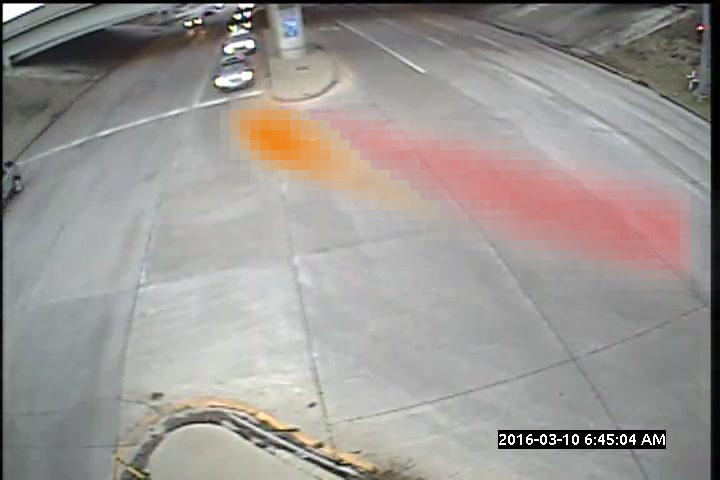
\includegraphics[width=\linewidth]{./img/scene_learning/topics/topic-1.jpg}
    \end{subfigure}%
    \begin{subfigure}{0.32\linewidth}
        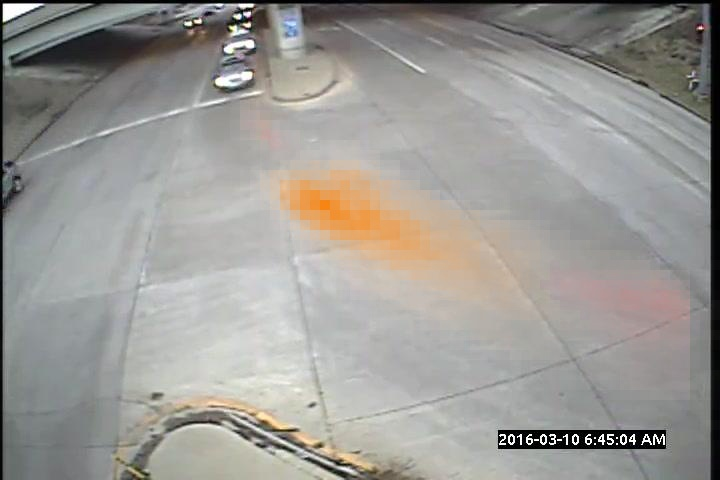
\includegraphics[width=\linewidth]{./img/scene_learning/topics/topic-3.jpg}
    \end{subfigure}%
    \begin{subfigure}{0.32\linewidth}
        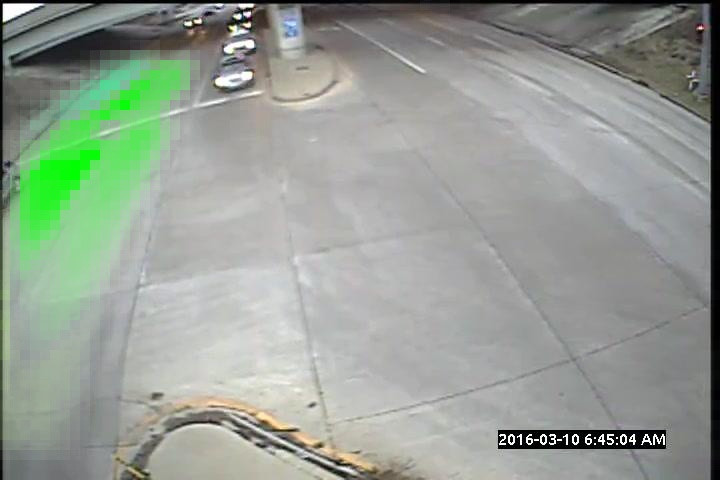
\includegraphics[width=\linewidth]{./img/scene_learning/topics/topic-0.jpg}
    \end{subfigure}%

    \begin{subfigure}{0.32\linewidth}
        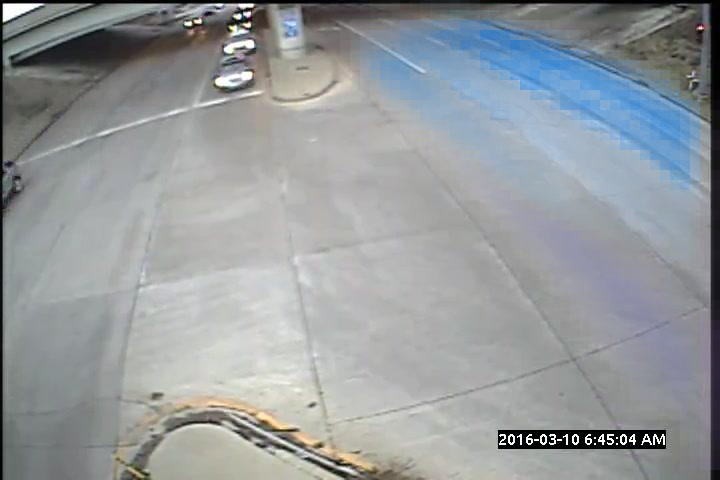
\includegraphics[width=\linewidth]{./img/scene_learning/topics/topic-2.jpg}
    \end{subfigure}%
    \begin{subfigure}{0.32\linewidth}
        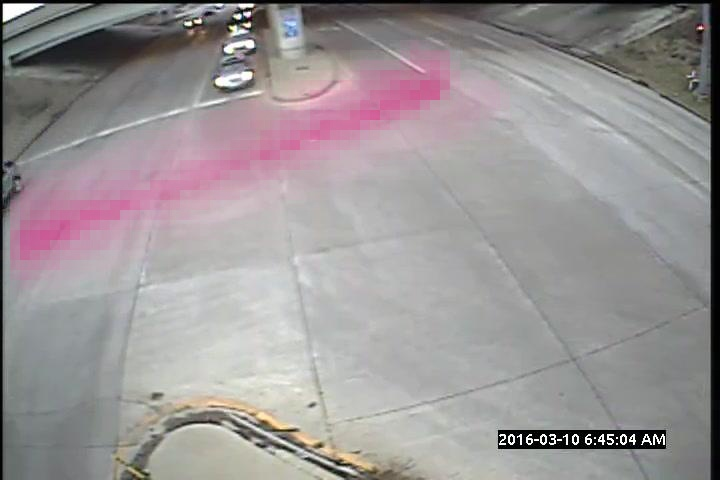
\includegraphics[width=\linewidth]{./img/scene_learning/topics/topic-4.jpg}
    \end{subfigure}%
    \hspace{0.08\linewidth}
    \begin{subfigure}{0.16\linewidth}
        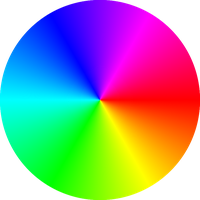
\includegraphics[width=\linewidth]{./img/scene_learning/color_wheel.png}
    \end{subfigure}
    \caption{Motions learned by HDP, colors indicate directions as the color wheel shows, the lightness indicate the magnitudes of the maximal probability values..}
    \label{fig:scene-topics}
\end{figure}